\documentclass{beamer}

\mode<presentation> {
	\usetheme{Madrid}
	\usecolortheme{default}
	\usepackage{textpos}
	\usefonttheme{default}
	\setbeamertemplate{caption}[numbered]
	\setbeamertemplate{itemize items}[circle]	%square, circle, etc, ...
	\setbeamertemplate{headline}{}				%removes top bar
	\setbeamertemplate{navigation symbols}{}	%remove navigation symbols
	%\setbeamerfont{frametitle}{size=\small}
}

\usepackage[english]{babel}
\usepackage[utf8x]{inputenc}
\usepackage{graphicx}
\usepackage{caption}
\usepackage{pgfplots}

\usepackage{clrscode3e}
\usepackage{natbib}


%\usepackage{array}
%\usepackage[framed,numbered,autolinebreaks,useliterate]{mcode}
%\usepackage{ragged2e}

\newcommand{\R}{\mathbb{R}}

\title[MIML]{Multi Instance Multi Label}
\titlegraphic{
\includegraphics[height=2cm,width=2cm]{headers/logo-unifi}}
\institute[]{{\large Machine Learning}\\\vspace{0.3cm}\textit{University of Florence, Department of Information Engineering}}
\author[L. Niccolai, F. Vittorini]
{\parbox[c]{1.5in}{Lorenzo Niccolai\\\texttt{\tiny lorenzo.niccolai3@stud.unifi.it}} \and 
\parbox[c]{1.5in}{Fabio Vittorini\\\texttt{\tiny fabio.vittorini@stud.unifi.it}}}
\date{\today}
\hypersetup{pdfauthor={Lorenzo Niccolai and Fabio Vittorini}}

%\AtBeginSection[] {
%	\begin{frame}{Contents}
%		\tableofcontents[currentsection]
%	\end{frame}
%}


\begin{document}
	
	
\frame[plain]{\titlepage} % Print the title page as the first slide

\usebackgroundtemplate
{
	%\includegraphics[width=\paperwidth,height=\paperheight]{background4}
}


%----------------------------------------------------------------------------------------
%	PRESENTATION SLIDES
%----------------------------------------------------------------------------------------

\begin{frame}{Overview}
	\tableofcontents
\end{frame}

\section{SVM}
\subsection{Classification}
\begin{frame}{Binary classification}
	\begin{itemize}\setlength\itemsep{1em}
		\item[Goal:] To produce a classifier able to decide whether an object belongs to one or more classes.
		\item[Idea:] Supervised Learning: Given a dataset of already classified examples, the classifier \textit{learns} a function that solves classification problem.
	\end{itemize}
\end{frame}

\begin{frame}{Notation}
	\begin{itemize}\setlength\itemsep{1em}
		\item A vector $x \in \mathbb{R}^f$ represents an object using $f$ \textit{relevant} features.
		\item A vector $y \in \{-1 , +1\}^l$ indicates wether the example belong to each of the $l$ label classes.
	\end{itemize}
	The input of a classification problem is a dataset $D = \{X, Y\}$ where $X \in \mathbb{R}^{n\times f}$ is a set of examples and $Y \in \mathbb{R}^{n\times l}$ is a set of labels.
	
	While learning the target function, the dataset is divided in \textit{training set} and \textit{test set}.
\end{frame}

\subsection{SVM idea}

\begin{frame}{SVM idea}
	\begin{itemize}\setlength\itemsep{1em}
		\item For 1-class problems we have to compute the \textit{maximum-margin hyperplane} $w^Tx + b$ which best separates positive examples from negative examples.
	\end{itemize}
	Optimization problem is:
	\begin{columns}
		\begin{column}{0.5\textwidth}\centering
			$$arg min_w \frac{1}{2} ||w||^2$$
			$$y^{(i)} (w^T x^{(i)} + b) \geq 1 \ \forall i \in [1, n]$$
		\end{column}
		\begin{column}{0.5\textwidth}\centering
			\begin{figure}[htbp]
				\centering
				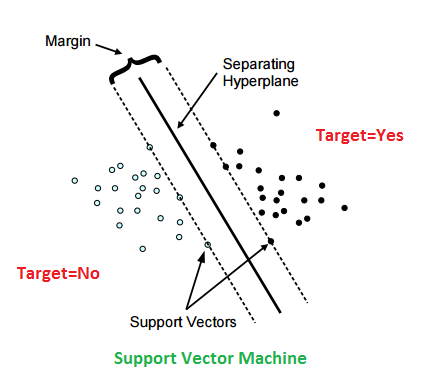
\includegraphics[scale = 0.40]{./images/optimal-hyperplane2.png}
				\caption{\textit{Solution of maximum-margin hyperplane}}
			\end{figure}
		\end{column}
	\end{columns}
	
	
	
\end{frame}

\begin{frame}{SVM idea}
	\begin{itemize}\setlength\itemsep{1em}
		\item The examples may not be linearly serparable and so the problem would not have any solutions because constraints are not satisfied. Then we introduce slack variables $\xi$
	\end{itemize}
	Optimization problem becames:
	\begin{columns}
		\begin{column}{0.5\textwidth}\centering
			$$arg min_{w, \xi} \frac{1}{2} ||w||^2 + C \sum_{i = 1}{n}\xi^{(i)}$$
			$$y^{(i)} (w^T x^{(i)} + b) \geq 1 - \xi^{(i)} \ \forall i \in [1, n]$$
			$$\xi^{(i)} \geq 0 \ \forall i \in [1, n]$$
		\end{column}
		\begin{column}{0.5\textwidth}\centering
			\begin{figure}[htbp]
				\centering
				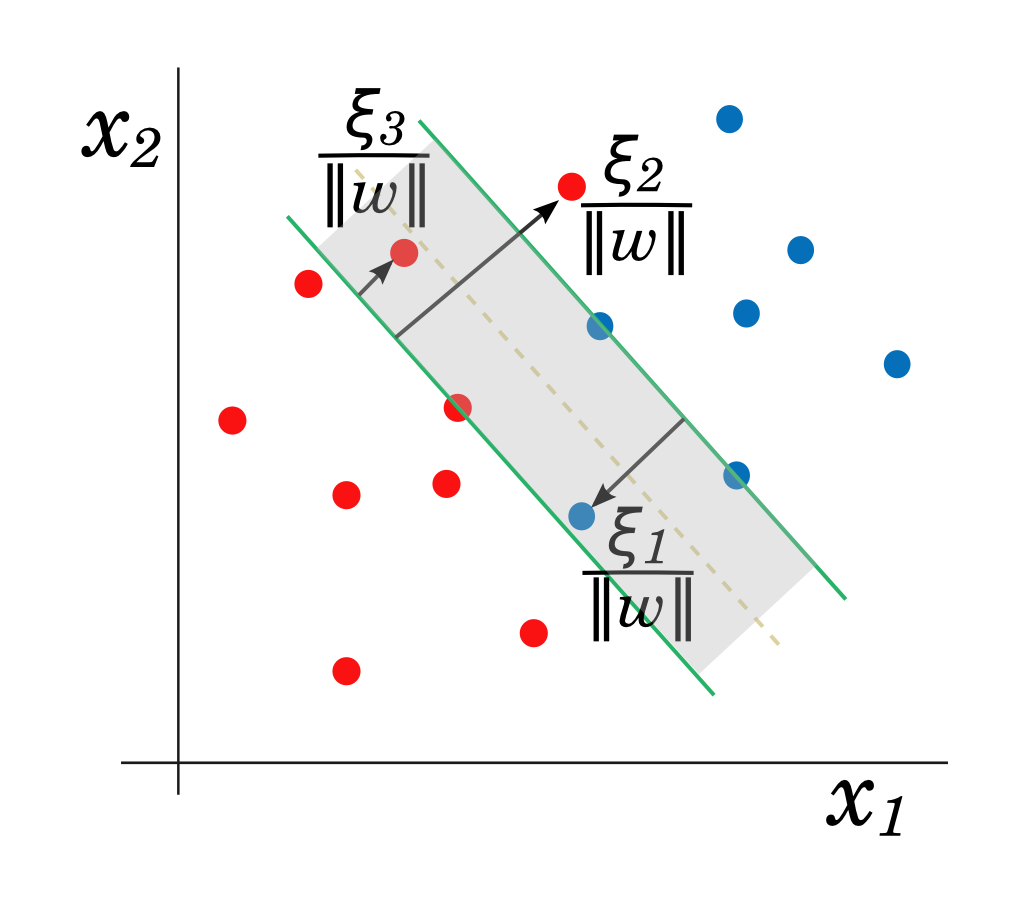
\includegraphics[scale = 0.15]{./images/slack2.png}
				\caption{\textit{Solution with slacks}}
			\end{figure}
		\end{column}
	\end{columns}
	
\end{frame}
\section{Multi Instance Learning}
 
\subsection{Introduction}
\begin{frame}{Multi instance classification}
	Motivation:
	\begin{itemize}\setlength\itemsep{1em}
		\item Sometimes a complex item can be well represented by a set of \textit{instances}
		\item A single instance may belong or not to a class
		\item An example is positive if at least one of its instances is positive, it's negative otherwise
		\item Dataset labels are assigned to examples, not to instances
		\item We have a \textit{semi-supervised learning} problem
	\end{itemize}
	\cite{mi1}
\end{frame}

\begin{frame}{Notation}
	Dataset is now a set of bags, where each bag is a set of instances:
	$$D = \{(X_i, Y_i) | i \in [1, n]\}$$
	$$X_i = \{x_{i,k} | k \in [1, k_i], x_{i,k} \in \R^f\}$$
	Notice that each bag can be made of any number of instances, but every instance has a fixed number of features $f$.
\end{frame}

\subsection{SIL}
\begin{frame}{SIL}
	The first naive approach makes the following label assignment:
	\begin{itemize}\setlength\itemsep{1em}
		\item If an instance belongs to a negative bag, sets its label to $-1$
		\item If an instance belongs to a positive bag, sets its label to $+1$
	\end{itemize}
	\vspace{5px}
	The resulting problem can be solved using a regular SVM, treating each instance as a whole document.\\
	\vspace{12px}
	Using this approach makes almost useless multi-instance formulation.
\end{frame}


\subsection{mi-SVM}
\begin{frame}{mi-SVM}
	Instances label assignment:
	\begin{itemize}\setlength\itemsep{1em}
		\item If an instance belongs to a negative bag we can say that its label is $-1$
		\item If an instance belongs to a positive bag we don't know for sure its label
	\end{itemize}
	\vspace{12px}
	This leads to 2 new constraints in SVM problem:
	$$y_{i,k} = -1 \ if \ Y_i = -1$$
	$$\sum_{k = 1}^{k_i}\frac{y_{i,k} + 1}{2} \geq 1 \ if \ Y_i = +1$$
\end{frame}

\begin{frame}{mi-SVM}
	Our SVM problem becames the following:
	$$min_Y min_{w, \xi} \frac{1}{2} ||w||^2 + C \sum_{i = 1}^{n}\xi_i$$
	$$y_{i,k} (w^T x_{i,k} + b) \geq 1 - \xi_i \ \forall i \in [1, n], k \in [1, k_i]$$
	$$\xi_i \geq 0 \ \forall i \in [1, n]$$
	$$y_{i,k} = -1 \ if \ Y_i = -1$$
	$$\sum_{k = 1}^{k_i}\frac{y_{i,k} + 1}{2} \geq 1 \ if \ Y_i = +1$$
	That is an intractable mixed optimization problem
\end{frame}

\begin{frame}{Algorithm}
	A feasible algorithm that finds a non optimal solution is the following:
	
	\begin{codebox}
		\Procname{$\proc{mi-SVM}\left(X, Y\right)$}
		\li $y_k^{(i)} = -1 \ if \ Y^{(i)} = -1$
		\li $y_k^{(i)} = +1 \ if \ Y^{(i)} = +1$
		\li \textbf{do} \Do
		\li Solve regular SVM finding $w$, $b$
		\li $y_k^{(i)} = sign(w^T x_k^{(i)} + b) \ if \ Y^{(i)} = +1$
		\li Adjust each positive bag to satisfy constraints \End
		\li \While($y_k^{(i)}$ change)
		
	\end{codebox}
	
\end{frame}

\subsection{MI-SVM}
\begin{frame}{MI-SVM}
	This approach uses directly the dataset in its bag form:
	$$arg min_{w, \xi} \frac{1}{2} ||w||^2 + C \sum_{i = 1}^{n}\xi^{(i)}$$
	$$y^{(i)} (max_k w^T x_k^{(i)} + b) \geq 1 - \xi^{(i)} \ \forall i \in [1, n]$$
	$$\xi^{(i)} \geq 0 \ \forall i \in [1, n]$$
	This is possible by selecting a \textit{witness} from each bag instances.
\end{frame}

\begin{frame}{Algorithm}
	A feasible algorithm that finds a solution is the following:
	
	\begin{codebox}
		\Procname{$\proc{MI-SVM}\left(X, Y\right)$}
		\li $\bar{x}_i = avg(x_{i,k}) \ \forall x_{i,k} \in X_i$ positive bag
		\li \textbf{do} \Do
		\li Assign $\bar{\alpha}_i \in [0,C]$ to each $\bar{x}_i$
		\li Assign $\alpha_{i,j}$ with $\sum_{j=1}^{k_i}\alpha_{i,j} \in [0,C] \ \forall x_{i,k} \in X_i$ negative bag
		\li Solve regular SVM finding $w$, $b$
		\li Find new $\bar{x}_i$ by selecting the best one for each positive bag \End
		\li \While(witnesses change)
		
	\end{codebox}
	
\end{frame}


 \section{Multi Label Learning}
 
\subsection*{Introduction}
\begin{frame}{Multi label classification}
	Motivation:
	\begin{itemize}\setlength\itemsep{1em}
		\item Sometimes a complex item can be well represented by a set of \textit{labels}
		\item Helps single label classification when the concept is more complicated or general
	\end{itemize}
	Solutions:
	\begin{itemize}\setlength\itemsep{1em}
		\item Problem transformation
		\item Algorithm adaptation
	\end{itemize}
\end{frame}

\begin{frame}{Notation}
	A set of labels $L = \{y_1, y_2,... y_l\}$ is given.\\
	Each object contained in the dataset is associated with a set of labels:
	$$D = \{(X_i, Y_i | i \in [1, n]\}$$
	$$X_i \in \R^f$$
	$$Y_i = \{y_{i,h} | h \in [1, h_i], y_{i,h} \in L, h_i \leq l\}$$
\end{frame}

\begin{frame}{Problem transformation}
	Attempt to convert the multilabel problem in a regular binary task.
	
	Two lossy methods:
	\begin{itemize}\setlength\itemsep{1em}
		\item Randomly discard each label information except one from each instance
		\item Remove instances that have actually more than one label
	\end{itemize}
	Other solutions:
	\begin{itemize}\setlength\itemsep{1em}
		\item Train a binary classifier for each existing combination of labels
		\item Train a binary classifier for each label (used in this work)
	\end{itemize}
\end{frame}

\begin{frame}{Algorithm adaptation}
	Regular algorithms are modified to support multi-label tasks.
	
	Sometimes they use problem transformation at the core.
	
	An example using SVM-related approach based on ranking and label set size prediction.
\end{frame}

\begin{frame}{Another multi label approch}
	
	\begin{flushright}
		\cite{ml1}
	\end{flushright}
\end{frame}
\section{Multi Instance Multi Label Learning}
 
\subsection{Introduction}
\begin{frame}{Introduction to MIML}
	MIML problems combine motivations of multi instance and multi label ones.
	
	Given a set of labels $L = \{y_1, y_2,... y_l\}$
	$$X_i = \{x_{i,k} | k \in [1, k_i], x_{i,k} \in \R^f\} Y_i = \{y_{i,h} | h \in [1, h_i], y_{i,h} \in L, h_i \leq l\}$$
	$$D = \{(X_i, Y_i) | i \in [1, n]\}$$
	\begin{figure}[htbp]
		\centering
		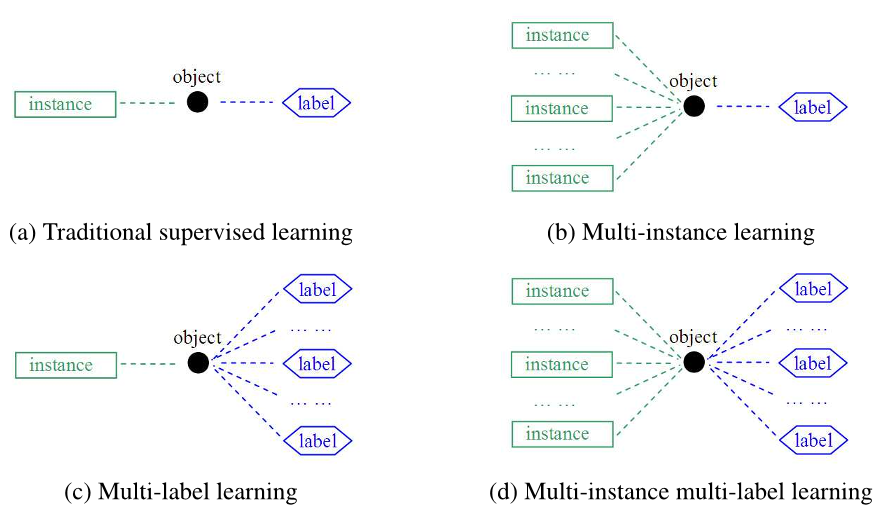
\includegraphics[scale = 0.25]{./images/confronto-miml.png}
		
	\end{figure}
	\cite{miml1}
\end{frame}

\begin{frame}{SVM Solution}
	To allow regular SVMs to solve this problem, we use \textit{problem transformation}.
	
	There are 2 possibilities:
	\begin{itemize}
		\item MIML $\rightarrow$ MISL $\rightarrow$ SISL (used in this work)
		\item MIML $\rightarrow$ SIML $\rightarrow$ SISL
	\end{itemize}
	\begin{figure}[htbp]
		\centering
		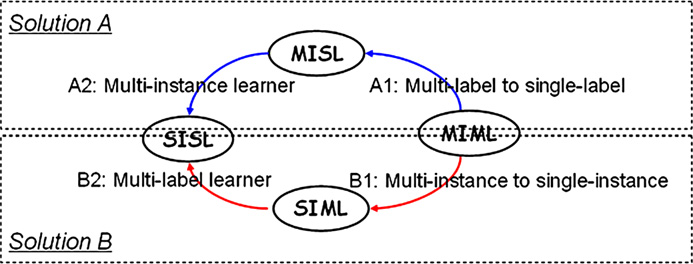
\includegraphics[scale = 0.40]{./images/2-metodi.png}
		
	\end{figure}
\end{frame}

\begin{frame}{Multi label to single label}
	Excluding lossy approaches, the idea is to train a multi-instance (single label) classifier for each label.
	
	Given a MIML dataset $D = \{(X_i, Y_i) | i \in [1, n]\}$	we produce $l$ datasets as follows:
	$$D_{y_j} = \{(X_i, Y_{y_j}) | i \in [1, n]\} \ \forall j \in [1, L]$$
	Where
	$$Y_{y_j} = 
	\begin{cases}
		+1 \ if \ y_j \in Y_i \\
		-1 \ otherwise
	\end{cases}$$
	Then we train $L$ regular multi-instance SVMs and collect their results.
\end{frame}

\begin{frame}{Multi instance to single instance}

	Given one of MISL datasets produced at previous step, we compared the 3 methods previously exposed:
	\begin{itemize}
		\item SIL
		\item MI-SVM
		\item mi-SVM
	\end{itemize}
	
	They all use a standard SISL SVM as subroutine.
\end{frame}

 


\begin{frame}[allowframebreaks]{References}
\bibliographystyle{plain}
\bibliography{sections/bibliography}
\end{frame}

\end{document} 